%=========================================================

% Here you can choose to compile with or without solutions.
% However, this definition is ignored if you use any
% command from the `Makefile`.
\providecommand{\withSol}{\iftrue}

%=========================================================

\documentclass
[twoside,german,colorbacktitle,accentcolor=tud9c]
{tudexercise}

\usepackage[T1]{fontenc}
\usepackage[utf8]{inputenc}
\usepackage[ngerman]{babel}
\usepackage{amstext}
\usepackage{amsmath}
\usepackage{graphicx}
\usepackage{setspace}
\usepackage{multicol}
\usepackage{mathtools}
\usepackage{dsfont}
\usepackage{units}
\usepackage{subfigure}
\usepackage{color}
\usepackage{booktabs}
\usepackage{fancyref}
\usepackage{gensymb}
\usepackage{tikz}
\usetikzlibrary{shapes.misc} 


%=========================================================


\setcounter{section}{1}
%=========================================================

\newcommand{\grp}{F}

%=========================================================


\begin{document}

\title{GDV 2 -- Theorie Übung \arabic{section}}
\subtitle{Winter Semester 2018/19}
\subsubtitle{Übungsgruppe \grp{}}

\maketitle

%=========================================================



\begin{examheader}
	\textmb{GDV 1 - Theorie Übung \arabic{section} | Gruppe \grp{}}\\
	\begin{tabular}{l l l l l}
		Moritz Fuchs	& Alexander Jäger	& Amon Ditzinger	& John Kalkhoff	\\
	\end{tabular}
\end{examheader} 


%=========================================================
% Anpassung an Aufgabenstellung
\renewcommand\thesubsection{Aufgabe \arabic{subsection}}
\renewcommand\thesubsubsection{\alph{subsubsection})}

%=========================================================
\newpage
\newif\ifvimbug
\vimbugfalse

\ifvimbug
\begin{document}
\fi


\subsection{Quantisierung von Positionsdaten (4 Punkte)}
\subsubsection{2 Punkte}
Quantiesierung für b=2. Erster Pfeil Quantisierung und zweiter Pfeil Dekomprimierung.\\
$\begin{pmatrix} 0\\1 \end{pmatrix} \rightarrow \begin{pmatrix} 2\\3 \end{pmatrix} \rightarrow \begin{pmatrix} 1/3\\1 \end{pmatrix}\\
\begin{pmatrix} -0.7\\-0.7 \end{pmatrix} \rightarrow \begin{pmatrix}0\\0 \end{pmatrix} \rightarrow \begin{pmatrix} -1\\-1 \end{pmatrix}\\
\begin{pmatrix} 0.7\\0.7 \end{pmatrix} \rightarrow \begin{pmatrix} 3\\3 \end{pmatrix} \rightarrow \begin{pmatrix} 1\\1 \end{pmatrix}\\
\begin{pmatrix} -1\\0 \end{pmatrix} \rightarrow \begin{pmatrix} 0\\2 \end{pmatrix} \rightarrow \begin{pmatrix} -1\\1/3 \end{pmatrix}\\
\begin{pmatrix} 1\\0 \end{pmatrix} \rightarrow \begin{pmatrix} 3\\2 \end{pmatrix} \rightarrow \begin{pmatrix} 1\\1/3 \end{pmatrix}\\
\begin{pmatrix} -0.7\\0.7 \end{pmatrix} \rightarrow \begin{pmatrix} 0\\3 \end{pmatrix} \rightarrow \begin{pmatrix} -1\\1 \end{pmatrix}\\
\begin{pmatrix} 0.7\\-0.7 \end{pmatrix} \rightarrow \begin{pmatrix} 3\\0 \end{pmatrix} \rightarrow \begin{pmatrix} 1\\-1 \end{pmatrix}\\
\begin{pmatrix} 0\\0 \end{pmatrix} \rightarrow \begin{pmatrix} 2\\2 \end{pmatrix} \rightarrow \begin{pmatrix} 1/3\\1/3 \end{pmatrix}\\
\begin{pmatrix} 0\\-1 \end{pmatrix} \rightarrow \begin{pmatrix} 2\\0 \end{pmatrix} \rightarrow \begin{pmatrix} 1/3\\-1 \end{pmatrix}\\$

Quantiesierung für b=3.\\
$\begin{pmatrix} 0\\1 \end{pmatrix} \rightarrow \begin{pmatrix}4\\7 \end{pmatrix} \rightarrow \begin{pmatrix} 1/7\\1 \end{pmatrix}\\
\begin{pmatrix} -0.7\\-0.7 \end{pmatrix} \rightarrow \begin{pmatrix}1\\1 \end{pmatrix} \rightarrow \begin{pmatrix} -5/7\\-5/7 \end{pmatrix}\\
\begin{pmatrix} 0.7\\0.7 \end{pmatrix} \rightarrow \begin{pmatrix} 6\\6 \end{pmatrix} \rightarrow \begin{pmatrix}5/7 \\5/7\end{pmatrix}\\
\begin{pmatrix} -1\\0 \end{pmatrix} \rightarrow \begin{pmatrix} 0\\4 \end{pmatrix} \rightarrow \begin{pmatrix} -1\\1/7 \end{pmatrix}\\
\begin{pmatrix} 1\\0 \end{pmatrix} \rightarrow \begin{pmatrix} 7\\4 \end{pmatrix} \rightarrow \begin{pmatrix} 1\\1/7 \end{pmatrix}\\
\begin{pmatrix} -0.7\\0.7 \end{pmatrix} \rightarrow \begin{pmatrix} 1\\6 \end{pmatrix} \rightarrow \begin{pmatrix} -5/7\\5/7 \end{pmatrix}\\
\begin{pmatrix} 0.7\\-0.7 \end{pmatrix} \rightarrow \begin{pmatrix} 6\\1 \end{pmatrix} \rightarrow \begin{pmatrix} 5/7\\-5/7 \end{pmatrix}\\
\begin{pmatrix} 0\\0 \end{pmatrix} \rightarrow \begin{pmatrix} 4\\4\end{pmatrix} \rightarrow \begin{pmatrix} 1/7\\1/7 \end{pmatrix}\\
\begin{pmatrix} 0\\-1 \end{pmatrix} \rightarrow \begin{pmatrix} 4\\0 \end{pmatrix} \rightarrow \begin{pmatrix} 1/7\\-1 \end{pmatrix}\\$

<<<<<<< HEAD
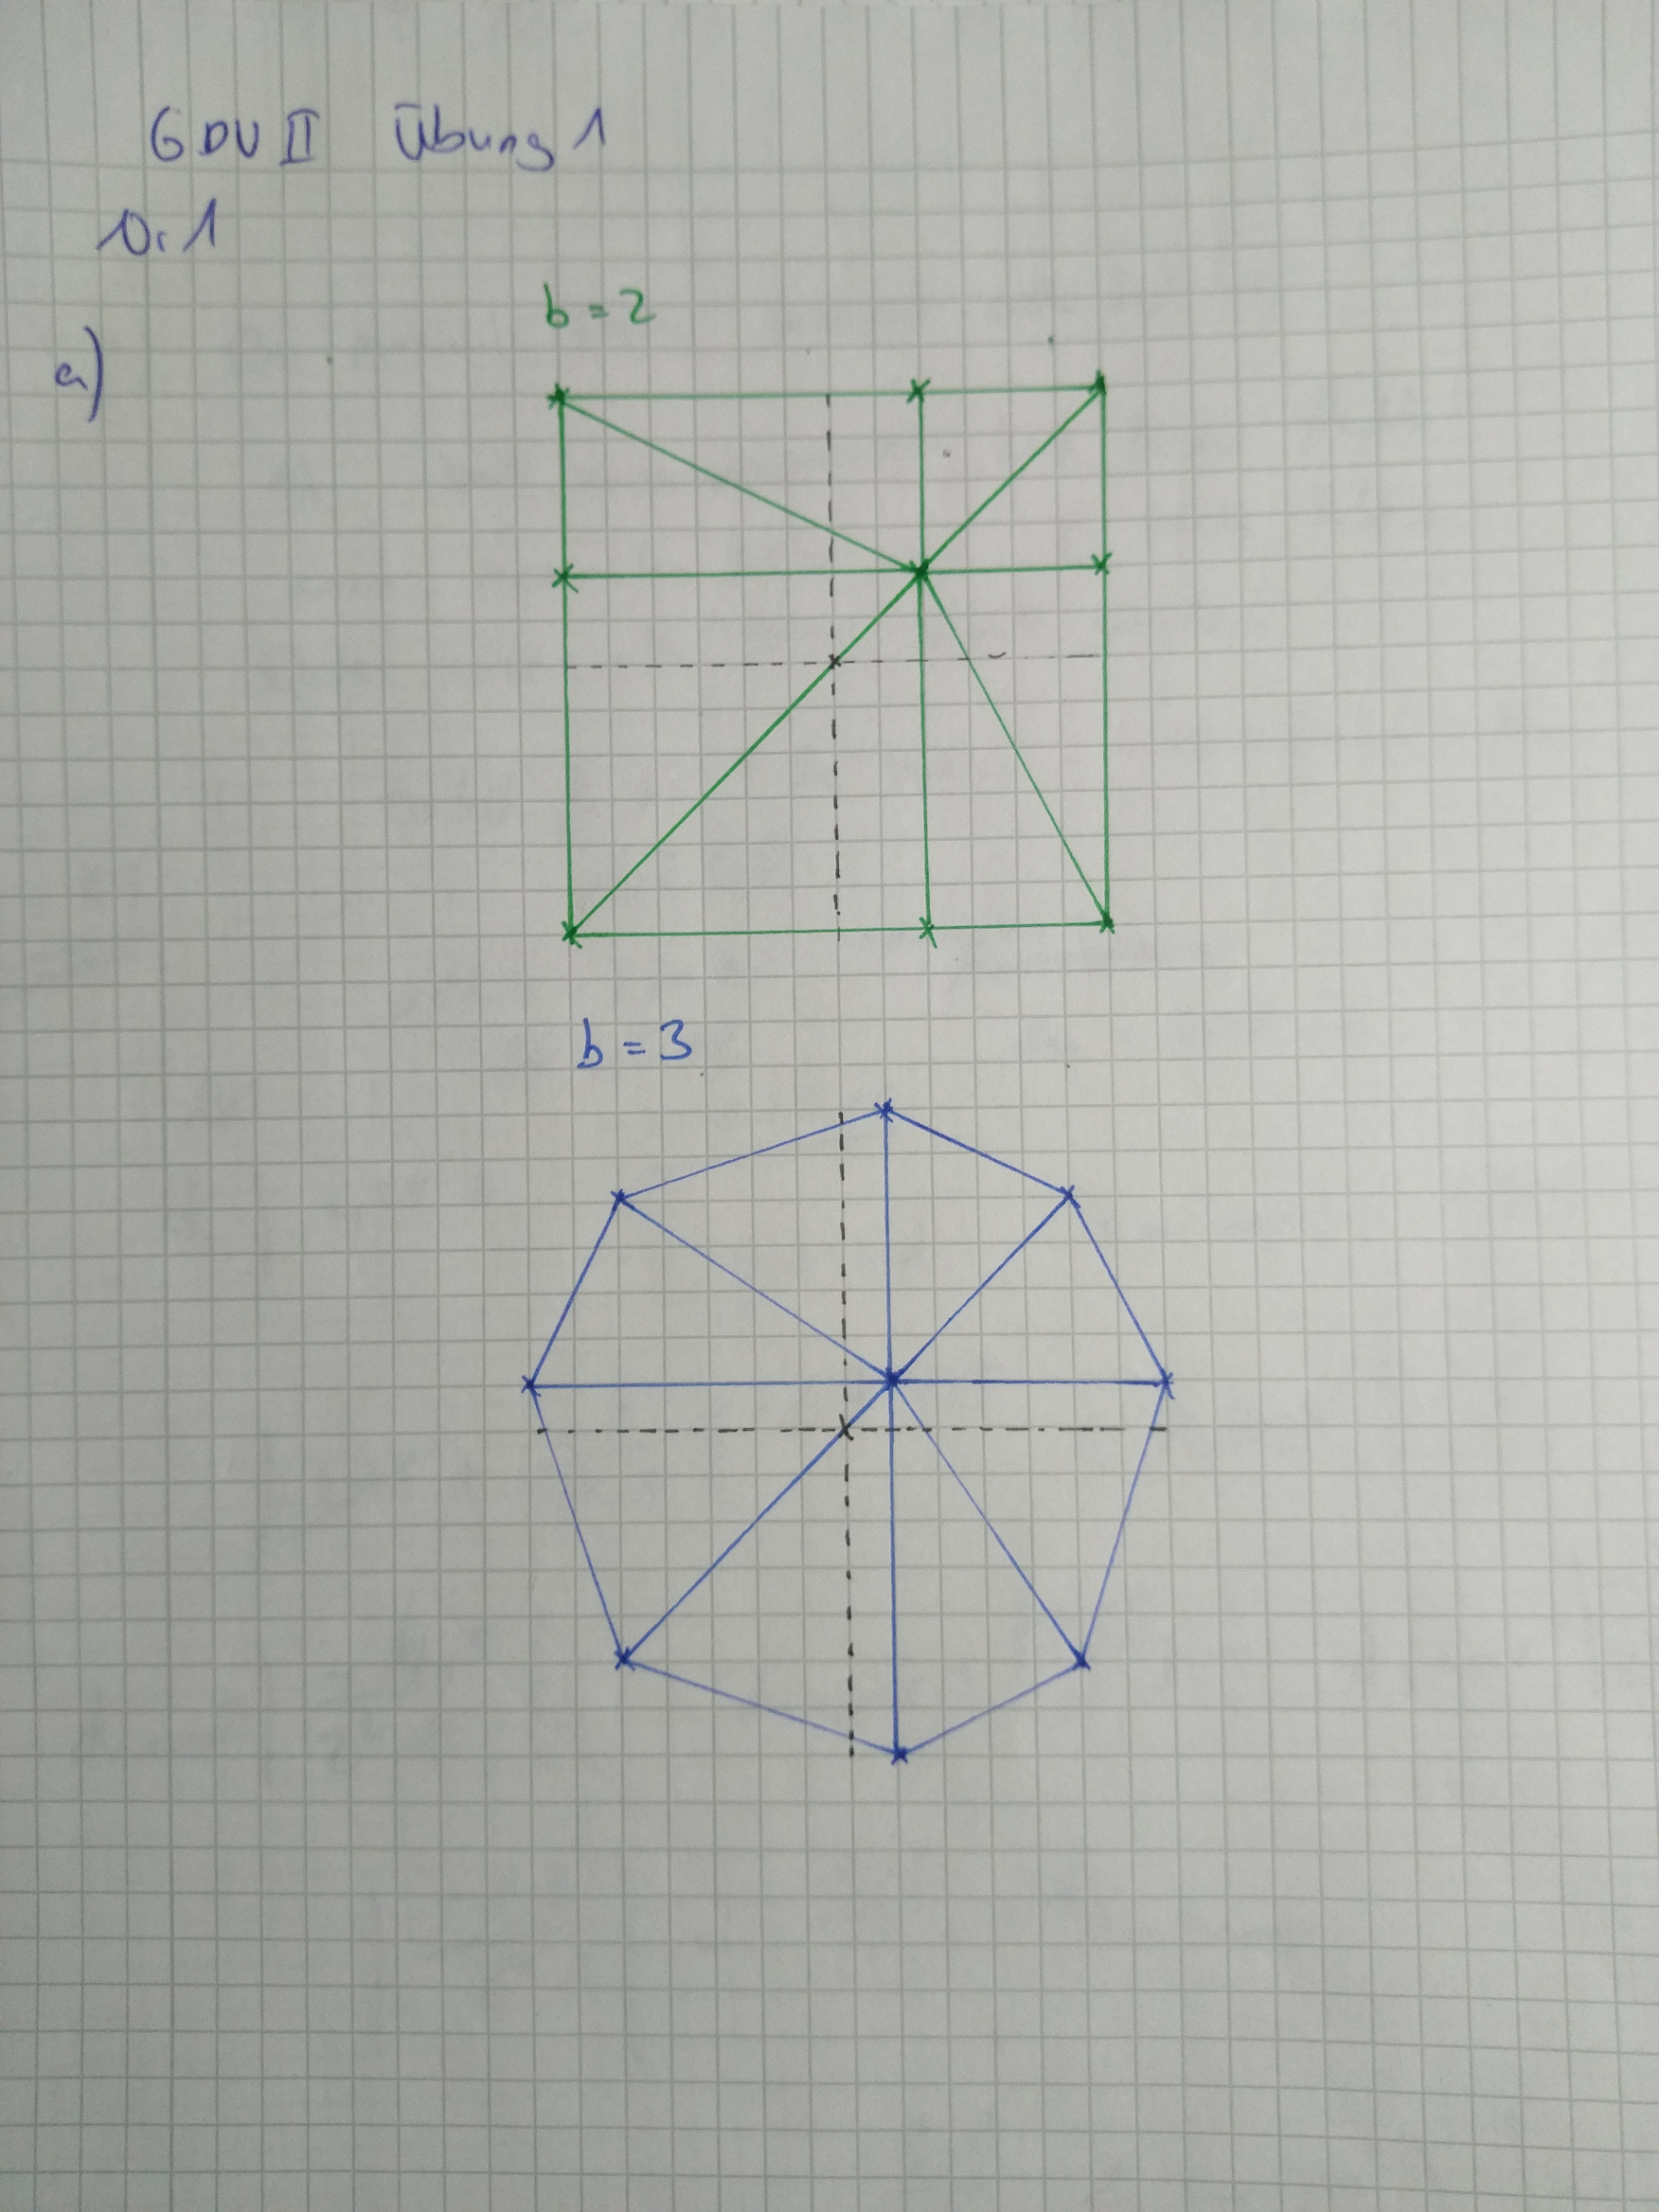
\includegraphics[scale=0.25]{1a_Zeichnung_J}

\subsubsection{2}
=======
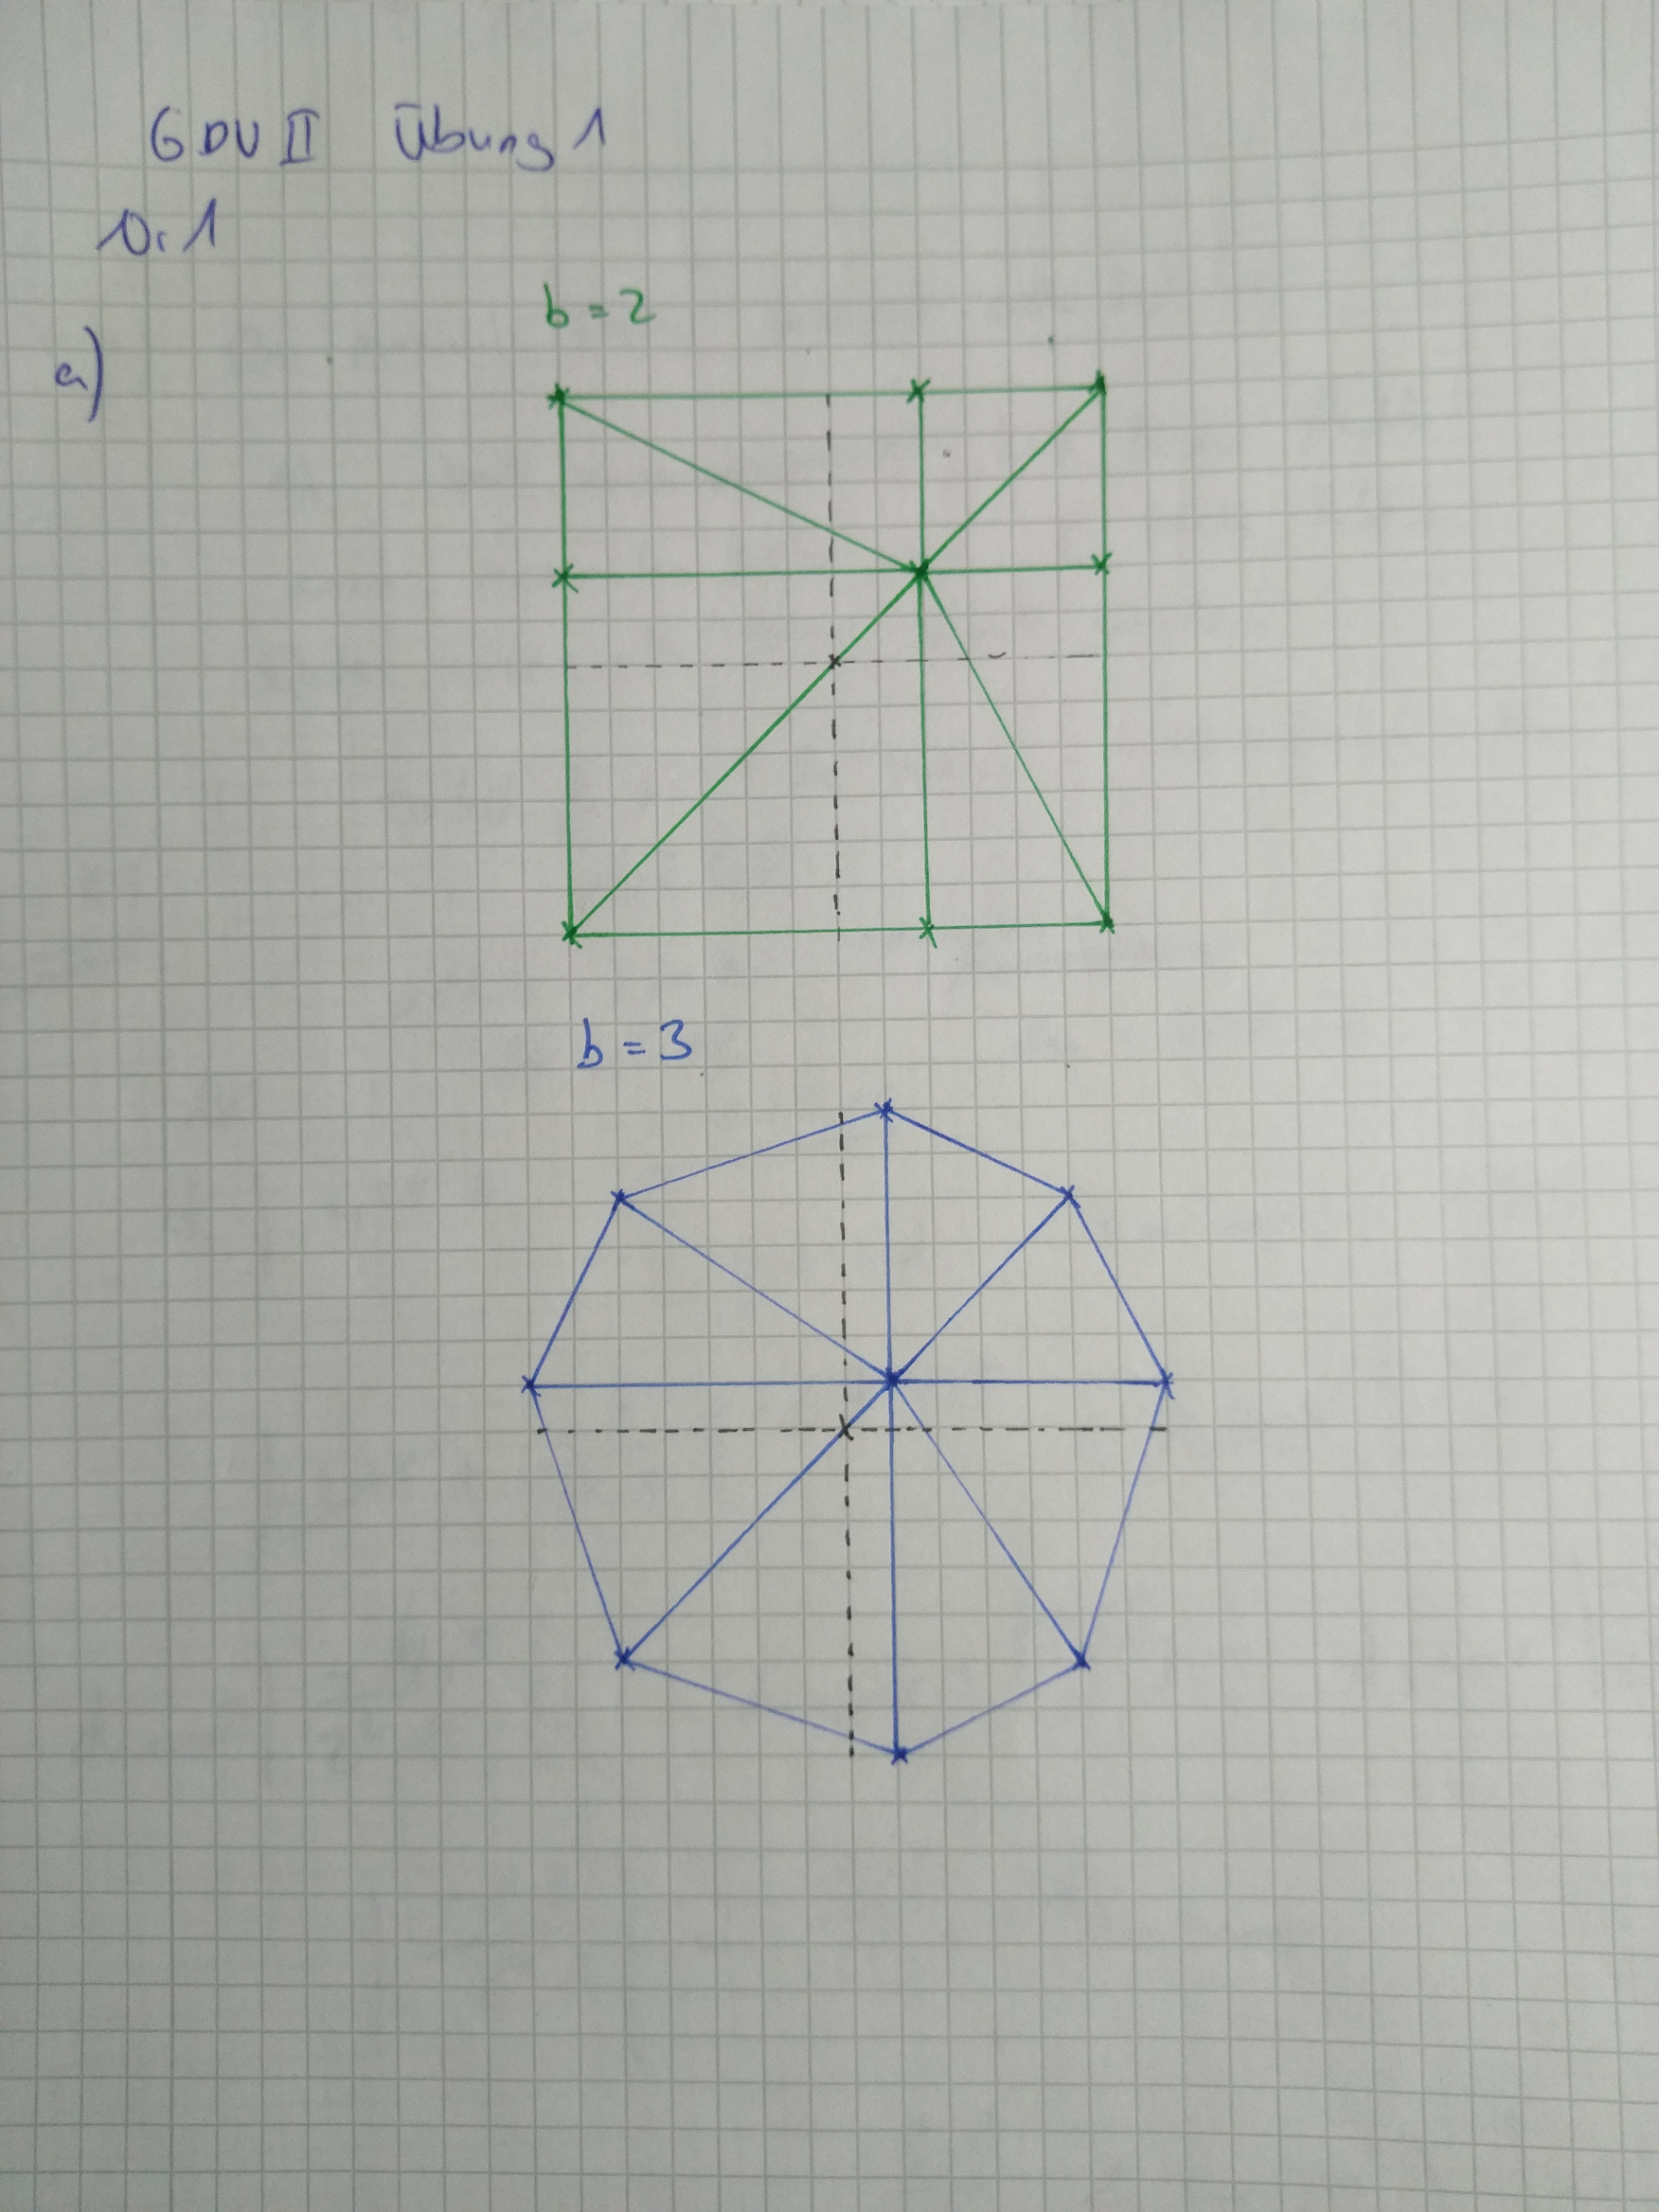
\includegraphics[height=9cm]{1a_Zeichnung_J.jpg}
>>>>>>> b9ce24dce1a570fcb0ae46d004a76d1d68135e22

\subsubsection{2 Punkte}
Ein Punkt $p$ mit einer $AABB(m,M)$ und Bildtiefe $b$ auf den Punkt $p*$. Daraus folgt das es ein $q\in[0.2^b-1]$ gibt, sodass $dekomprimierung(q) = p_q = p^*$. Der maximale Fehler entsteht nun wenn ein Nachbarpunkt $p_{q+1}$ dekomprimiert wird. Der Abstand von $p_q$ un $p_{q+1}$ ist:\\
$$|p_{q+1}-p_q|_2 = |\frac{1}{2^b-2^0}(M-m)|_2$$
$p$ wird auf $q$ abgebildet wird, folgt das $p$ auf $p^*$ abgebildet damit gilt für den maximalen Fehler:\\
$$Fehler_{kompression} = | p - p^*|_2 \leq |\frac{1}{2} \frac{1}{2^b-2^0}(M-m)|_2 $$
Der mittlere Fehler ist dann die Hälfte davon.
\subsubsection{1 Punkt}
$$ 0.5 \leq \frac{1}{2} \frac{1}{2^b-2^0}\cdot5450 $$\\
$$ 1 \leq  \frac{1}{2^b-2^0}\cdot5450$$\\
$$ \frac{1}{5450} \leq  \frac{1}{2^b-2^0}$$\\
$$ 5450 \geq  2^b-1$$\\
$$ 5451 \geq  2^b$$\\
$$ \log(5451) \geq  \log(2)\cdot b$$\\
$$ \approx 12,45 \geq  b$$\\
Damit werden mindestens 13 Bit benötigt.



\newpage
\newif\ifvimbug
\vimbugfalse

\ifvimbug
\begin{document}
\fi


\subsection{Octahedron Normalen Kompression (5 Punkte)}
\subsubsection{1}

\subsubsection{2}

\subsubsection{1}





%=========================================================

\end{document}
